\documentclass{beamer}
\usepackage{amsmath}
\usepackage{gvv}

\title{Question 4.2.3}
\author{AI25BTECH11040 - Vivaan Parashar}
\date{\today}

\begin{document}

\frame{\titlepage}

\begin{frame}
    \frametitle{Question: }
    Find the direction and normal vectors of each of the following line: $-2x + 3y = 6$
\end{frame}

\begin{frame}
    \frametitle{Solution: }
    Assuming points on the line are represented by $\vec{x}$, we can express the line equation as:
    \begin{align}
        \norm{\myvec{-2 \\ 3}^{\mathrm{T}}\vec{x}} = 6
    \end{align}
    In such a form, the normal vector $\vec{n}$ is given by:
    \begin{align}
        \vec{n} = \myvec{-2 \\ 3} \equiv \frac{1}{\sqrt{13}}\myvec{2 \\ -3}
    \end{align}
    The direction vector $\vec{d}$ can be derived from the normal vector by rotating it by 90 degrees clockwise (or anticlockwise). To do that, we multiply with the transformation matrix $\vec{r}$:
    \begin{align}
        \vec{r} = \myvec{0                             & 1 \\ -1 & 0}\\
        \therefore \vec{d} = \vec{r}\vec{n} = \myvec{0 & 1 \\ -1 & 0}\myvec{-2 \\ 3} = \myvec{-3 \\ -2} \equiv \frac{1}{\sqrt{13}}\myvec{3 \\ 2}
    \end{align}
\end{frame}

\begin{frame}
    \frametitle{Plot: }
    \begin{figure}[h!]
        \centering
        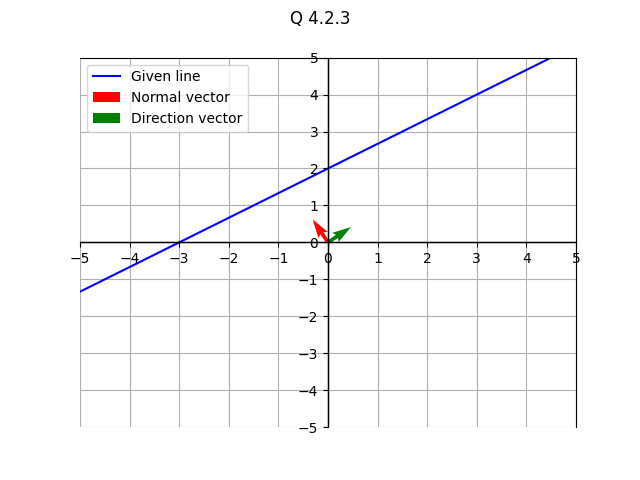
\includegraphics[width=0.9\columnwidth]{../figs/plot.png}
        \caption{Graph of line with direction and normal vectors}
        \label{fig:4.2.3}
    \end{figure}
\end{frame}

\end{document}
